\documentclass[twoside]{article}
\setlength{\oddsidemargin}{0 in}
\setlength{\evensidemargin}{0 in}
\setlength{\topmargin}{-0.6 in}
\setlength{\textwidth}{6.5 in}
\setlength{\textheight}{8.5 in}
\setlength{\headsep}{0.75 in}
\setlength{\parindent}{0 in}
\setlength{\parskip}{0.1 in}

\usepackage{url}
\usepackage{titlesec}
\setcounter{secnumdepth}{3}
\usepackage{palatino}
\usepackage{marginnote}
\usepackage{multirow}
\usepackage{easybmat,bigdelim,arydshln}
\usepackage[authoryear,round]{natbib}
\usepackage{amssymb,amsmath,amsthm,amsfonts}
\usepackage{mathtools}
\usepackage{caption}
\usepackage{hyperref}
\usepackage{tcolorbox}
\tcbuselibrary{skins, breakable, theorems}
\usepackage{newpxtext,newpxmath}
\usepackage{longtable}
\usepackage{enumitem}
\makeatletter

\let\bar\overline

\setlist[itemize]{topsep=0pt,leftmargin=10pt,itemsep=-0.2em}
\usepackage{xcolor}
\usepackage{tikz}
\usepackage{pgfplots}
\pgfplotsset{compat = newest}
\usetikzlibrary{patterns,decorations.pathreplacing,decorations.markings}
\usepgfplotslibrary{fillbetween}

\hypersetup{
    colorlinks,
    citecolor=red,
    filecolor=black,
    linkcolor=violet,
    urlcolor=blue
}

\definecolor{myblue}{cmyk}{1,.72,0,.38}
\definecolor{mypurple}{cmyk}{.57,1,0,.58}
\definecolor{myred}{cmyk}{0,.88,.88,.58}
\definecolor{mygreen}{cmyk}{1,0,.69,.66}
\definecolor{myorange}{cmyk}{0,.58,100,.20}

\makeatletter
\renewcommand{\thefigure}{\thesection.\arabic{figure}}
\newtheoremstyle{indented}
  {3pt}% space before
  {3pt}% space after
  {\addtolength{\@totalleftmargin}{3.5em}
   \addtolength{\linewidth}{-3.5em}
   \parshape 1 3.5em \linewidth}% body font
  {}% indent
  {\bfseries}% header font
  {.}% punctuation
  {.5em}% after theorem header
  {}% header specification (empty for default)
\makeatother

\theoremstyle{definition}
\newtheorem{defin}{Definition}[section] % Creates a new counter, number within section
\newtheorem{prt}[defin]{Remark} 
\newtheorem{prts}[defin]{Remarks} % Again share defin's counter
\newtheorem{exmp}[defin]{Example} % etc.
\newtheorem{exmps}[defin]{Examples}
\newtheorem*{note}{Note}
\tcbuselibrary{theorems}

% use counter*=defin to make each tcbtheorem share defin's counter

\newtcbtheorem[use counter*=defin, number within=section]{definition}{Key takeaways}{enhanced, breakable,
    colback = white, colframe = myred, colbacktitle = red!55!black, attach boxed title to top left = {yshift = -2.5mm, xshift = 3mm}, boxed title style = {sharp corners},fonttitle=\bfseries}{takeaway}

\newtcbtheorem[use counter*=defin, number within=section]{theorem}{Theorem}{enhanced, breakable,
    colback = white, colframe = myblue, colbacktitle = blue!45!black, attach boxed title to top left = {yshift = -2.5mm, xshift = 3mm}, boxed title style = {sharp corners},fonttitle=\bfseries}{thm}
    
\newtcbtheorem[use counter*=defin, number within=section]{proposition}{Proposition}{enhanced, breakable,
    colback = white, colframe = teal, colbacktitle = teal, attach boxed title to top left = {yshift = -2.5mm, xshift = 3mm}, boxed title style = {sharp corners},fonttitle=\bfseries}{prop}

\newtcolorbox{example}[1]{enhanced, breakable, colback = white, colframe = orange!85!black, colbacktitle = orange!85!black, attach boxed title to top left = {yshift = -2.5mm, xshift = 3mm}, boxed title style = {sharp corners},fonttitle=\bfseries, title={Example: #1}}

\newtcbox{\myhl}[1][white]
  {on line, arc = 0pt, outer arc = 0pt,
    colback = #1!20!white, colframe = #1!50!black,
    boxsep = 0pt, left = 1pt, right = 1pt, top = 1pt, bottom = 1pt, boxrule = 0pt, bottomrule =0pt, toprule =0pt}
    
\newtcbox{\myhlrule}[1][white]
  {on line, arc = 0pt, outer arc = 0pt,
    colback = #1!20!white, colframe = #1!50!black,
    boxsep = 0pt, left = 1pt, right = 1pt, top = 1pt, bottom = 1pt, boxrule = 0pt, bottomrule =0.5pt, toprule =0.5pt}
%
% The following commands set up the lecnum (lecture number)
% counter and make various numbering schemes work relative
% to the lecture number.
%
\newcounter{lecnum}
\renewcommand{\thepage}{\thelecnum-\arabic{page}}
\renewcommand{\thesection}{\thelecnum.\arabic{section}}
\renewcommand{\theequation}{\thelecnum.\arabic{equation}}
\renewcommand{\thefigure}{\thelecnum.\arabic{figure}}
\renewcommand{\thetable}{\thelecnum.\arabic{table}}

\newcommand{\sidenotes}[1]{\marginnote{\raggedright\scriptsize#1}}
%
% The following macro is used to generate the header.
%
\newcommand{\lecture}[4]{
   \pagestyle{myheadings}
   \thispagestyle{plain}
   \newpage
   \setcounter{lecnum}{#1}
   \setcounter{page}{1}
   \noindent
   \begin{center}
   \framebox{
      \vbox{\vspace{2mm}
    \hbox to 6.28in { {\bf ECON203: Principles of Microeconomics
	\hfill Fall 2022} }
       \vspace{4mm}
       \hbox to 6.28in { {\Large \hfill Note #1: #2  \hfill} }
       \vspace{2mm}
       \hbox to 6.28in { {\it Lecturer: #3 \hfill TA: #4} }
      \vspace{2mm}}
   }
   \end{center}
   \markboth{Week #1: #2}{Week #1: #2}

   {\bf Key points}: {\begin{itemize}
       \item Don't be afraid of math, plug in numbers and try, maybe it's not that difficult.
       \item Elasticity is very confusing, but always remember that both the denominator and the numerator are \textbf{percentage} changes.
       \item If something doesn't add up, draw a graph.
   \end{itemize}}

   {\bf Disclaimer}: {\it These notes are written by Sai Zhang for ECON203, based on the problem sets written by Prof. Brijesh Pinto, the instructor of the course. Please do \textbf{NOT} distribute them online without permission.}
   \vspace*{4mm}
}
%

\tikzset{-stealth-/.style={decoration={
  markings,
  mark=at position #1 with {\arrow{stealth}}},postaction={decorate}}}

  \tikzset{tangent/.style={
    decoration={
        markings,% switch on markings
        mark=
            at position #1
            with
            {
                \coordinate (tangent point-\pgfkeysvalueof{/pgf/decoration/mark info/sequence number}) at (0pt,0pt);
                \coordinate (tangent unit vector-\pgfkeysvalueof{/pgf/decoration/mark info/sequence number}) at (1,0pt);
                \coordinate (tangent orthogonal unit vector-\pgfkeysvalueof{/pgf/decoration/mark info/sequence number}) at (0pt,1);
            }
    },
    postaction=decorate
},
use tangent/.style={
    shift=(tangent point-#1),
    x=(tangent unit vector-#1),
    y=(tangent orthogonal unit vector-#1)
},
use tangent/.default=1}

\begin{document}
\lecture{2}{Questions in PS3 and PS4}{Brijesh Pinto}{Sai Zhang}

\section{Utility maximization problem (UMP)}

For this part of the discussion, we focus on the case of 2 goods: $x,y$.

\subsection{Indifference curves}

For a utility function
$$
u(x,y) = xy
$$

we replace $u(x,y)$ with the value of utility to be achieved to get the family of indifference curves, that is:

\begin{center}
    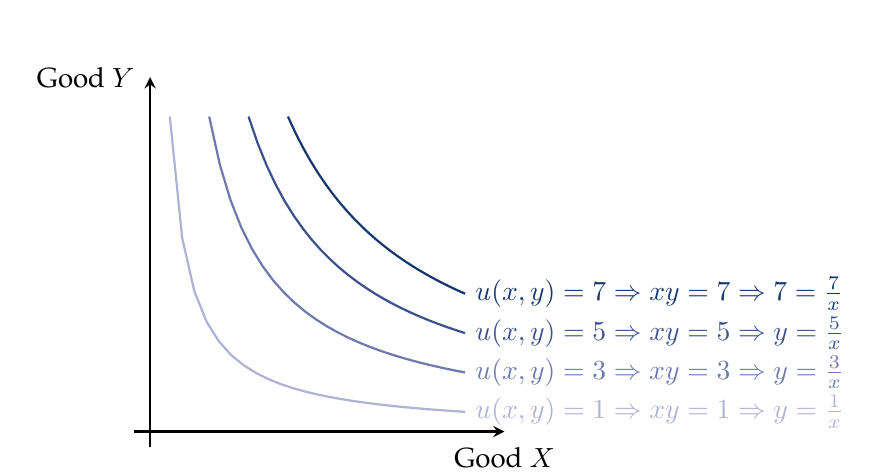
\begin{tikzpicture}[scale=1]
    % basics
    \draw [-stealth,color=black,thick] (-0.2,0) -- (4.5,0) node[below=2pt] {Good $X$};
    \draw [-stealth,color=black,thick] (0,-0.2) -- (0,4.5) node[left=2pt] {Good $Y$};
    
    \draw[domain=0.25:4, myblue!25!white, thick, variable=\x] plot ({\x}, {1/\x}) node[right] {$u(x,y)=1\Rightarrow xy=1 \Rightarrow y=\frac{1}{x}$};
    \draw[domain=0.75:4, myblue!50!white, thick, variable=\x] plot ({\x}, {3/\x}) node[right] {$u(x,y)=3 \Rightarrow xy=3 \Rightarrow y=\frac{3}{x}$};
    \draw[domain=1.25:4, myblue!75!white, thick, variable=\x] plot ({\x}, {5/\x}) node[right] {$u(x,y)=5\Rightarrow xy=5 \Rightarrow y=\frac{5}{x}$};
     \draw[domain=1.75:4, myblue, thick, variable=\x] plot ({\x}, {7/\x}) node[right] {$u(x,y)=7 \Rightarrow xy=7 \Rightarrow 7=\frac{7}{x}$};
    
\end{tikzpicture}
\end{center}

Then you can derive a function $y=f(x)$, and determine the shape (convex/concave, downward-/upward-sloping, horitonal/vertical, etc) of the family of indifference curves.

\subsection{Budget constraints}
Always remember to start from the basic:
$$
p_x x + p_y y = I
$$
with some math transformation, we get a line:
$$
y = -\frac{p_x}{p_y} x + \frac{I}{p_y}
$$
plot this line:
\begin{center}
    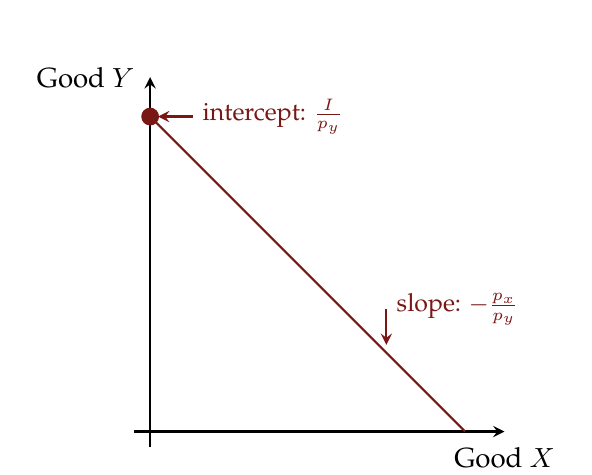
\begin{tikzpicture}[scale=1]
    % basics
    \draw [-stealth,color=black,thick] (-0.2,0) -- (4.5,0) node[below=2pt] {Good $X$};
    \draw [-stealth,color=black,thick] (0,-0.2) -- (0,4.5) node[left=2pt] {Good $Y$};
    
    \draw[domain=0:4, myred, thick, variable=\x] plot ({\x}, {4-\x});
    
    \filldraw[myred] (0,4) circle (3pt); 
    
    % text
    \draw[-stealth,thick,myred] (0.55,4) -- node[right=6pt] {\small intercept: $\frac{I}{p_y}$} (0.1,4);
    \draw[stealth-,thick,myred] (3,1.1) --  (3,1.55) node[right] {\small slope: $-\frac{p_x}{p_y}$};
    
\end{tikzpicture}
\end{center}

So given different sets of information, what can we infer?
\begin{itemize}
    \item[-] slope and intercepts given: we know slope $\left(-\frac{p_x}{p_y}\right)$ and intercept $\left(\frac{I}{p_y}\right)$, we can \textbf{NOT} determine the prices ($p_x,p_y$) or the income level ($I$), because we only know the ratios.
    \item[-] 2 points on the line given: if we know 2 points on the budget line, we can only determine the slope and the intercept of the line. Hence, same as the first scenario, we can \textbf{NOT} determine the level of $p_x,p_y,I$.
\end{itemize}

To summarize: 
\begin{itemize}
    \item[-] if we have the information about the budget line itself (its slope, intercepts, or any 2 points on it), we can \textbf{only} infer: \myhl[myred]{price ratio $\frac{p_x}{p_y}$ (given by slope), and $\frac{I}{p_y}$}. To determine the \textbf{level} of $p_x,p_y,I$, we need to know at least one of them in addition to the budget line information.
    \item[-] On the other hand, if we know the price ratio $\frac{p_x}{p_y}$, we know the slope of the budget line. If we also know a point on the line, or the intercept of the line, we can determine the budget  line itself (like in PS3 Q6).
\end{itemize}

\subsection{Utility maximization}

What should we do when facing questions like Q8-Q10 in PS3? Here's a general way of thinking.

Use Q8 of PS3 as an example, the information we have:
\begin{itemize}
    \item[-] $I=20,p_x=2,p_y=4$, or the budget line: $2x+4y=20\Rightarrow y =-\frac{1}{2}x+5$
    \item[-] the MRS at point $(x=4,y=3)$: $MRS_{(4,3)}=1$
\end{itemize}

\subsubsection*{Intuitive way}
The intuition is quite simple:
\begin{itemize}
    \item[-] the budget line tells us: to buy \myhl[myblue]{\textbf{1} unit of $x$}, we need to give up \myhl[myred]{\textbf{0.5} unit of $y$}, since $\frac{p_x}{p_y}=\frac{1}{2}$\footnote{Remember? This is the (absolute value of the) slope.}.
    \item[-] $MRS=1$, which means that at $(x=4,y=3)$, \myhl[myblue]{\textbf{1} extra unit of $x$} is equivalent (in regards to the utility they generate) to \myhl[myred]{\textbf{1} extra unit of $y$}\footnote{Remember the definition of $MRS$? It's \textbf{marginal}, that's why I say \textbf{extra unit}}.
\end{itemize}
Now as we write things down, it's pretty clear that at $(x=4,y=3)$, $\frac{p_x}{p_y}<MRS$, that is:

\begin{quote}
    One extra unit of $x$ and one extra unit of $y$ generate the same level of utility, but one extra unit $x$ is cheaper!
\end{quote}

So to maximize your utility, you would want to buy \textbf{more} of $x$. 

\subsubsection*{Graphic way}
We can also draw a graph to illustrate. Remember MRS at a bundle is the \textbf{slope} of the \textbf{tangent line} to the indifference curve at that point, then we can draw

\begin{center}
    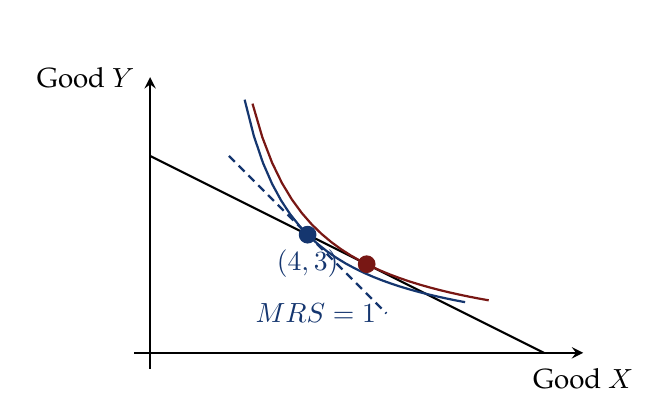
\begin{tikzpicture}[scale=1]
    % basics
    \draw [-stealth,color=black,thick] (-0.2,0) -- (5.5,0) node[below=2pt] {Good $X$};
    \draw [-stealth,color=black,thick] (0,-0.2) -- (0,3.5) node[left=2pt] {Good $Y$};
    
    % walrasian
    \draw[domain=0:5, black, thick, variable=\x] plot ({\x}, {2.5-0.5*\x});
    \draw[domain=1:3, myblue, thick, densely dashed, variable=\x] plot ({\x}, {3.5-\x}) node[left] {$MRS=1$};
    \draw[domain=1.2:4, myblue, thick, variable=\x] plot ({\x}, {2.25/(\x-0.5)});
    \draw[domain=1.3:4.3, myred, thick, variable=\x] plot ({\x}, {2.25^2/(2*(\x-0.5))});
    
    % intersection: \bar{p}
    \filldraw[myblue] (2,1.5) circle (3pt) node[below=2pt] {$(4,3)$}; 
    \filldraw[myred] (2.75,2.5-2.75/2) circle (3pt); 
    
\end{tikzpicture}
\end{center}

It's easy to see that: by moving from the blue bundle $(x=4,y=3)$ to the red bundle ($x\uparrow,y\downarrow$), we get a higher level of utility (the red indifference curve is above the blue one, indicating a higher utility level).

\myhl[myblue]{\textbf{One more thing!}} Always check whether the given bundle is on the budget line \textbf{first}! If it's below the line:
\begin{itemize}
    \item[-] you want to buy more of $x$ and more of $y$ when the MRS at the given bundle \textbf{equals} the absolute value of the slope
    \item[-] otherwise, not sure.
\end{itemize}

\section{Demand function and elasticity}
\subsection{Horizontal sum of demand functions}
This type of question is not as tricky as you might think, let's break it down. There are 2 scenarios to consider: the 2 demand curves have 
\begin{itemize}
    \item[-] same y-axis intercepts
    \item[-] different y-axis intercepts
\end{itemize}

\begin{center}
\begin{minipage}[b]{0.45\textwidth}
    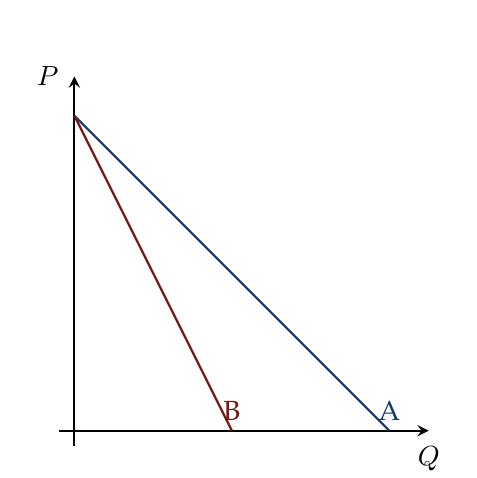
\begin{tikzpicture}[scale=1]
         % basics
    \draw [-stealth,color=black,thick] (-0.2,0) -- (4.5,0) node[below=2pt] {$Q$};
    \draw [-stealth,color=black,thick] (0,-0.2) -- (0,4.5) node[left=2pt] {$P$};
    
    % walrasian
    \draw[domain=0:4, myblue, thick, variable=\x] plot ({\x}, {4-\x}) node[above] {A};
    \draw[domain=0:2, myred, thick, variable=\x] plot ({\x}, {4-2*\x}) node[above] {B};
    \end{tikzpicture}
  \end{minipage}
  \hfill
  \begin{minipage}[b]{0.45\textwidth}
    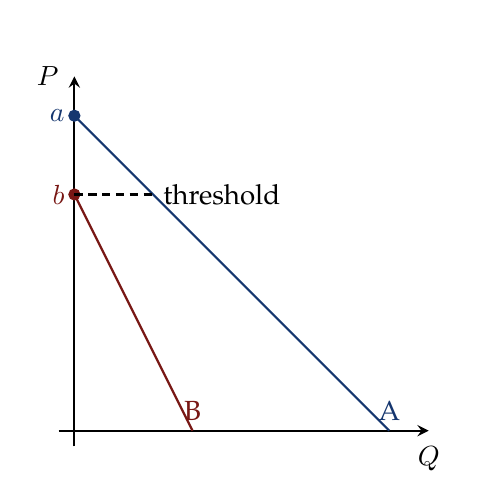
\begin{tikzpicture}[scale=1]
        % basics
    \draw [-stealth,color=black,thick] (-0.2,0) -- (4.5,0) node[below=2pt] {$Q$};
    \draw [-stealth,color=black,thick] (0,-0.2) -- (0,4.5) node[left=2pt] {$P$};
    
    \filldraw[myblue] (0,4) circle (2pt) node[left] {$a$};
    \filldraw[myred] (0,3) circle (2pt) node[left] {$b$};
    
    % walrasian
    \draw[domain=0:4, myblue, thick, variable=\x] plot ({\x}, {4-\x}) node[above] {A};
    \draw[domain=0:1.5, myred, thick, variable=\x] plot ({\x}, {3-2*\x}) node[above] {B};
    \draw[thick, densely dashed, black] (0,3) -- (1,3) node[right] {threshold};
    \end{tikzpicture}
  \end{minipage}
\end{center}

\subsubsection*{Same y-axis intercepts (left graph)}
Conceptually, this is a simpler case: 

We use the setting of PS4-Q3, that is, adding $P=a-eQ$ and $P=a-fQ$. Since the 2 lines have the same y-axis intercepts, we can just do the following:

\begin{itemize}
    \item[-] \myhl[myred]{\textbf{Step 1}:} write Q as a function of P:
    \begin{align*}
        P&=a-eQ\Rightarrow  Q=\frac{a-P}{e} & P&=a-fQ\Rightarrow Q=\frac{a-P}{f}
    \end{align*}
    
    \item[-] \myhl[myred]{\textbf{Step 2}:} add the right-hand wide of these two equations together, get the aggregate demand:
    $$
    Q = \frac{a-P}{e}+\frac{a-P}{f} = \frac{(e+f)(a-P)}{ef}
    $$
    
    \item[-] \myhl[myred]{\textbf{Step 3}:} rewrite this equation, expressing $P$ as a function of Q:
    \begin{align*}
        Q=\frac{(e+f)(a-P)}{ef} \Rightarrow \frac{ef}{e+f}Q=a-P \Rightarrow P= a-\frac{ef}{e+f}Q
    \end{align*}
\end{itemize}
Then, you have the horizontal sum of these two lines!

\subsubsection*{Different y-axis intercepts (right graph)}
This is a slightly more complicated scenario, but it's not that difficult. We only have one more thing to consider: when will the two agents (corresponding to the 2 demand curves) enter the market. Let's assume:
\begin{align*}
    \text{For A: } & P=a-eQ\\
    \text{For B: } & P= b-fQ
\end{align*}
and $0<b<a$.

\begin{itemize}
    \item[-] \myhl[myblue]{\textbf{Step 1}}: Determine when each of the two agents enter the market:
    
    In the graph (right panel), above the threshold,  the price is too high or $B$, hence only $A$ enters the market, the horizontal sum of $A$ and $B$ is just the demand of $A$, that is, the horizontal sum is $P=a-eQ$, when $b \leq P\leq a$.
    
    \item[-] \myhl[myblue]{\textbf{Step 2}}: below the threshold, repeat what we have done for the 1st scenario, to solve the horizontal sum:
    \begin{itemize}
        \item[1] for A: $P=a-eQ\Rightarrow Q=\frac{a-P}{e}$; for B: $P=b-fQ\Rightarrow Q=\frac{b-P}{f}$
        \item[2] sum the right-hand side: $Q=\frac{a-P}{e}+ \frac{b-P}{f} = \frac{(a-P)f+(b-P)e}{ef} = \frac{af+be}{ef}- \frac{e+f}{ef}P$
        \item[3] transform back: $P = -\frac{ef}{e+f}Q + \frac{af+be}{e+f}$
    \end{itemize}
    remember, we are looking at below-threshold, that is $0\leq P\leq b$.
\end{itemize}

See? Easy.

\section{Elasticity}
Last but not least, we look at elasticity. First, let's go over the deduction of at-a-point elasticity on a linear demand curve $P=a-mQ$:

\begin{align*}
    \epsilon = \frac{\frac{Q_2-Q_1}{Q_1}}{\frac{P_2-P_1}{P_1}} = \frac{Q_2-Q_1}{P_2-P_1}\cdot\frac{P_1}{Q_1} = -\frac{1}{m}\cdot \frac{P_1}{Q_1} \Rightarrow \left\vert\epsilon\right\vert = \frac{1}{m}\cdot\frac{P_1}{Q_1} = \frac{1}{m}\cdot\frac{a-mQ_1}{Q_1} = \frac{a}{mQ_1}-1
\end{align*}

Two properties to keep in mind:
\begin{itemize}
    \item[1] a linear demand curve cannot have a constant elasticity ($\epsilon$ changes as $Q_1$ changes).
    \item[2] for a linear demand curve, the absolute value of elasticity goes down if $Q_1$ goes up\footnote{This property is used for Q10 of PS4.}.
\end{itemize}

Elasticity can be quite a confusing concept, so let's look at it in a better-organized way. Again, we assume a linear demand curve $P=a-mQ$:
\begin{table}[h!]
\centering
    \begin{tabular}{c|c}
         elasticity & formula \\
        \hline
        own-price elasticity: at-a-point & $\lvert\epsilon\rvert=\frac{a}{mQ_1}-1$ \\
        own-price elasticity: mid-point & $\lvert\epsilon \rvert = \frac{1}{m}\cdot\frac{P_1+P_2}{Q_1+Q_2}$ \\
        cross-price {\footnotesize(demand for $x$ w.r.t. price of $y$)} elasticity ($P_x$ given) & $\lvert\epsilon \rvert=\frac{\frac{Q_{2,x}-Q_{1,x}}{(Q_{2,x}+Q_{1,x})/2}}{\frac{P_{2,y}-P_{1,y}}{(P_{2,y}+P_{1,y})/2}}$\\
        income elasticity ($P$ given) & $\lvert\epsilon \rvert=\frac{\frac{Q_{2}-Q_{1}}{(Q_{2}+Q_{1})/2}}{\frac{I_{2}-I_{1}}{(I_{2}+I_{1})/2}}$
    \end{tabular}
\end{table}

Some things to notice:
\begin{itemize}
    \item[-] for own-price elasticity: both at-a-point and mid-point calculation have the property that $Q\downarrow \Rightarrow \lvert\epsilon\rvert\uparrow$
    \item[-] remember that elasticity reflects the relative \textbf{percentage} change, so both the denominator and the numerator must be a \textbf{percentage} change.
    \item[-] elasticity and the 3 sets of goods:
    \begin{itemize}
        \item[-] own-price elasticity: the good is
        \begin{itemize}
            \item[$\cdot$] luxury: higher $\lvert\epsilon\rvert$, more price-elastic
            \item[$\cdot$] necessity: lower $\lvert\epsilon\rvert$, less price-elastic
        \end{itemize}
        \item[-] cross-price elasticity: the two goods are\footnote{Remember? The demand for the two goods move in the opposite directions if they are substitutes ($\Delta Q_1\Delta Q_2<0$); the demand for the two goods move in the same direction if they are compliments ($\Delta Q_1\Delta Q_2>0$).}
        \begin{itemize}
            \item[$\cdot$] substitutes:  $\epsilon >0$
            \item[$\cdot$] compliments: $\epsilon <0$
        \end{itemize}
        \item[-] income elasticity: the good is
        \begin{itemize}
            \item[$\cdot$] normal good: $\epsilon>0$
            \item[$\cdot$] inferior good: $\epsilon<0$
        \end{itemize}
    \end{itemize}
\end{itemize}

Hope this summary is useful for you, but you don't need to remember everything, all you need to remember is the law of demand $\Delta P\cdot \Delta Q<0$, and some intuitions.

\vspace{20pt}
\noindent\rule{\textwidth}{0.4pt}

\textbf{For fun}: what demand function has constant at-a-point elasticity? It's this family of function: 
$$
P=AQ^{\frac{1}{\epsilon}}
$$
where $\epsilon$ is the constant at-a-point elasticity. This family of functions looks like this:

\begin{center}
    \begin{tikzpicture}[scale=1]
    % basics
    \draw [-stealth,color=black,thick] (-0.2,0) -- (4.5,0) node[below=2pt] {$Q$};
    \draw [-stealth,color=black,thick] (0,-0.2) -- (0,4.5) node[left=2pt] {$P$};
    
    \draw[domain=0.75:4, myblue, thick, variable=\x] plot ({\x}, {3/\x});
\end{tikzpicture}
\end{center}


%\newpage
%\bibliographystyle{plainnat}
%\bibliography{ref.bib}

\end{document}